\section{TWIn Neural Networks for Sentinel data}
论文 Combining Sentinel-1 and Sentinel-2  Satellite Image Time Series for land cover mapping via a multi-source deep learning architecture~\cite{TWINNS} 的总结

\subsection{Introduction}
\paragraph*{para01---para03
    \textcolor[RGB]{17, 205, 29}{近年来全球发射大量卫星, 地球观测计划(Earth Observation),  哨兵一号二号卫星介绍. 主要包括卫星类型, 重访周期, 分辨率等参数.}}
\begin{quotation}
    \itshape
    In recent years, monitoring the Earth surface has become possible thanks to the development of several modern Earth Observation (EO) systems continuously providing massive amounts of satellite data. 
    
    A notable example is represented by the Copernicus programme developed by the European Space Agency (ESA), consisting of several constellations of satellites (i.e., the Sentinel missions), which monitor different aspects of the Earth Surface. In the context of area monitoring tasks, the Sentinel-1 (S1) and Sentinel-2 (S2) missions are of particular interest, since they provide publicly available radar (S1) and optical/multi-spectral (S2) satellite imagery with an high revisit time. The Sentinel-1 mission (composed of two satellites, Sentinel-1A and Sentinel-1B) is operating day and night, performing dual polarization C-band synthetic aperture radar (SAR) imaging acquired at a global scale in Terrain Observation with Progressive Scan (TOPS) mode with a re-visit period of 6 days. 
    
    The Sentinel-2 mission involves a constellation of two twin satellites (Sentinel-2A and Sentinel-2B), supplying optical information ranging from visible to near and medium infrared with a spatial resolution between 10 m and 20 m with a revisit period between 5 and 10 days.
\end{quotation}

\paragraph*{para04
    \textcolor[RGB]{17, 205, 29}{重访周期短, 空间分辨率高使卫星影像时间序列(Satellite Image Time Series)可用于生态学, 农业, 流动性分析, 风险评估, 城乡规划等研究领域.}}
\begin{quotation}
    \itshape
    Thanks to the high revisiting period, such high spatial resolution satellite images can be effectively organized in Satellite Image Time Series (SITS), which represent a practical tool to monitor Earth Surface evolution through time, supporting a wide number of application domains. For this reason, SITS have been successfully exploited to address tasks related to ecology (Kolecka et al., 2018; Chen et al., 2014), agriculture (Bégué et al., 2018; Bellón et al., 2017; Kussul et al., 2017), mobility, health, risk assessment (Olen and Bookhagen, 2018), land management planning (Inglada et al., 2017), forest (Wulder et al.,2012; Wulder et al., 2008) and natural habitat monitoring (Guttler et al., 2017; Khiali et al., 2018).
\end{quotation}

\paragraph*{para05
    \textcolor[RGB]{17, 205, 29}{单独使用哨兵一号卫星卫星遥感影像时间序列, 单独使用哨兵二号卫星遥感影像时间序列已经在土地覆盖方面有一定研究(应用).}}
\begin{quotation}
    \itshape
    In recent years, Sentinel-1 and Sentinel-2 SITS have been successfully exploited in the context of Land Use/Land Cover (LULC) mapping, demonstrating how the availability of such radar and optical SITS is beneficial in this domain. Some notable examples include the use of optical S2 SITS to produce land cover maps at country scale (Inglada et al., 2017) and to characterize grassland areas as a proxy indicator for biodiversity, food production, and global carbon cycle (Kolecka et al., 2018). Radar S1 SITS have also been effectively applied to different
    LULC-related tasks, such as analyzing the impact of seasonality in urban land cover mapping (Zhou et al., 2018) and mapping the quality of the land cover in winter season (Minh et al., 2018).
\end{quotation}

\paragraph*{para06
    \textcolor[RGB]{17, 205, 29}{作者认为现在最大的挑战是如何结合哨兵二号提供的光学影像和哨兵一号SAR影像. 并通过引证文献说明现阶段在融合使用哨兵一号哨兵二号影像在绿地变化监测, 变化检测, 森林野火和水生物入侵监测等方面融合光学和雷达影像效果是优于单影像. 并且作者认为哨兵一号影像与哨兵二号影像可以在某些方面形成互补}}
\begin{quotation}
    \itshape
    An attractive challenge in the remote sensing community is how to effectively combine the properties of surface materials provided by the optical sensor (S2) and the structural characteristics of landscape elements provided by the radar sensor (S1), i.e., two aspects that can be considered complementary with respect to the land cover mapping task. Combinations of optical and radar data have shown to perform better than the single sensors in different scenarios, such as grassland (Dusseux et al., 2014) and crop (Betbeder et al., 2014) monitoring, change detection (Gao et al., 2017), urban mapping (Iannelli and Gamba, 2018), wildfire assessment (Colson et al., 2018) and detection of invasive plants (Rajah et al., 2018).
\end{quotation}

\paragraph*{para07
    \textcolor[RGB]{17, 205, 29}{作者就本文研究内容的土地利用/土地覆盖介绍了多数据源的研究方法, 认为他们使用传统机器学习算法做土地利用, 虽证明了多源影像比使用单一影像效果好, 但其融合时并未考虑数据之间的关联性, 只是做了简单的串联(concatenation). }}
\begin{quotation}
    \itshape
    As regards LULC mapping, several approaches focus on data fusion techniques, i.e., on the opportunity to integrate the information contained in radar and optical data before processing it (Joshi et al., 2016). In Sharma et al. (2018) S1 images are combined with Landsat-8 optical images in order to produce an enhanced forest cover composite (i.e., by suppressing the green component over the non-forested vegetative areas). In Fernández-Beltran et al. (2018) a multimodal image fusion approach based on Latent Semantic Analysis is proposed, in order to deal with unsupervised land-cover mapping. In general LULC tasks, proposed approaches have often exploited standard machine learning techniques (i.e., Random Forest, SVM) on a simple concatenation of radar and optical input data (Steinhausen et al., 2018; Denize et al., 2019; Tricht et al., 2018; Lu et al., 2018; Hedayati and Bargiel, 2018; Erinjery et al., 2018; Whyte et al., 2018) without really leveraging the interplay between these two sources of information. Even though these approaches already prove how combining radar and optical data can improve performance over the use of a single sensor, they treat the two data sources as completely independent from each other. Furthermore, standard approaches ignore both spatial and temporal dependencies that may be present in the data, and they do not explicitly leverage the complementarity carried out by radar and optical SITS.
\end{quotation}

\paragraph*{para08
    \textcolor[RGB]{17, 205, 29}{引入深度学习用于遥感时序影像的研究现状. 经典的或是早期研究中常用的深度神经网络模型有两大类, 侧重于挖掘图像空间信息的卷积神经网络模型CNN和侧重于挖掘时序信息的循环神经网络模型RNN.}}
\begin{quotation}
    \itshape
    Models based on artificial neural networks, i.e., deep learning based models, are gaining attention in the remote sensing domain (Zhang and Du, 2016; Kussul et al., 2017; Zhu et al., 2017; Ienco et al., 2017; Lyu et al., 2016). The main attractive of these models is that they are able to learn features from the input data optimized for a specific task (e.g.,image classification), by simultaneously training the associated classifier. Moreover, they can be exploited to discover spatial as well as temporal dependencies in SITS. Most commonly used deep learning models are convolutional (Zhang and Du, 2016) (CNNs) and recurrent (Bengio et al., 2013) (RNNs) neural networks, which focus respectively on the analysis of spatial and temporal information in the data.
\end{quotation}

\paragraph*{para09
    \textcolor[RGB]{17, 205, 29}{近期研究有学者将RNN和CNN结合, 提出可处理时空数据的convRNN模型, 既可以挖掘时序信息也可挖掘空间特征. convRNN刚刚应用在遥感领域. 所引文献使用convRNN模型, 应用于哨兵二号的时序影像, 做语义分割. [单一时序影像, convRNN]}}
\begin{quotation}
    \itshape
    Recently, approaches incorporating both recurrent and convolutional operations were also proposed to deal with spatio-temporal data (Shi et al., 2015), namely convRNN models (e.g., ConvGru or ConvLSTM). Those architectures extend recurrent neural networks including convolutional operations in the recurrent unit and working on sequences of multi-dimensional data instead of sequences of vectors. These solutions are starting to get attention in the field of remotesensing, for instance, in Rußwurm and Körner (2018) the authors propose to use convRNN to tackle land cover classification from a Sentinel-2 SITS modeling the task as semantic segmentation (Volpi and Tuia, 2017).
\end{quotation}

\paragraph*{para10
    \textcolor[RGB]{17, 205, 29}{深度学习在融合影像刚刚开始, 还有很大的研究空间. 作者引证了使用CNN在多影像的应用. [多影像, CNN]}}
\begin{quotation}
    \itshape
    Combinations of optical and radar satellite images based on Deep learning techniques have been proposed to address tasks such as optical image simulation (He and Yokoya, 2018), change detection (Liu et al., 2018) and river discharge estimation (Tarpanelli et al.,2019). Nevertheless, the same opportunity has not been fully exploited yet in the context of LULC classification tasks. A first attempt has been made in Kussul et al. (2017), where stacked Sentinel-
    1 and Landsat-8 satellite images are used to feed a CNN-based classifier. However, the proposed CNN-based approach is rather simple, as it does not take into account temporal dependencies, and does not fully exploit the opportunity to learn features from radar and optical data separately.
\end{quotation}

\paragraph*{para11
    \textcolor[RGB]{17, 205, 29}{总结前两段, para09: convRNN只用于单一的时序影像; para10: 多源影像只使用了CNN. 因此本文提出的TWINN模型在多源影像中使用convRNN模型做时空信息挖掘. TWINN模型在数据互补主要体现在两方面: 一是可在不同源影像中互补; 二是可挖掘同源影像的时空数据.}}
\begin{quotation}
    \itshape
    In a previous work (Interdonato et al., 2019), we have shown how an architecture based on the combination of CNN and RNN models can help to leverage both spatial and temporal dependencies in optical SITS, thus being beneficial for LULC mapping tasks. In this work, our ambition is to introduce a further level of interaction based on the use of SITS coming from multiple sensors. The proposed TWINNS (TWIn Neural Networks for Sentinel data) architecture, is in fact devised to boost the land cover classification task by exploiting two levels of complementarity: the one between radar (S1) and optical (S2) satellite images, and the one between spatial and temporal dependencies in each image type. While the former point is possible due to the fact that specific and complementary per-source features are extracted, the latter point is addressed by exploiting Convolutional as well as Recurrent Neural Networks to manage spatial autocorrelation and temporal dependencies, respectively.
\end{quotation}

\subsection{Data}
研究的地区有两个. 

一是留尼汪岛, 它是印度洋西部马斯克林群岛中的火山岛. 为法国的海外省之一, 即留尼汪省. 留尼汪岛面积2512平方公里, 海岸线长207公里. 原始数据为2016年4月到2017年5月, 24张哨兵一号影像和34张哨兵二号影像. 二是Koumbia, 它是布基纳法索的一个农业自治镇. 原始数据为2016年1月到2016年12月的29张哨兵一号影像和23张哨兵二号影像. 

之后介绍了哨兵一号与哨兵二号影像的预处理. 留尼汪岛数据集和Koumbia数据集的构成. [奇怪的是, 这一部分有两段几乎一摸一样.] 真值来自于已有且与使用数据做过精密空间匹配的GIS数据库.

\subsection{TWINNS}
此部分为模型介绍, 共有两个分支和损失函数三个部分组成. [具体细节目前了解不是很清楚, 学习中.]
\begin{figure}[!htbp]
    \centering
    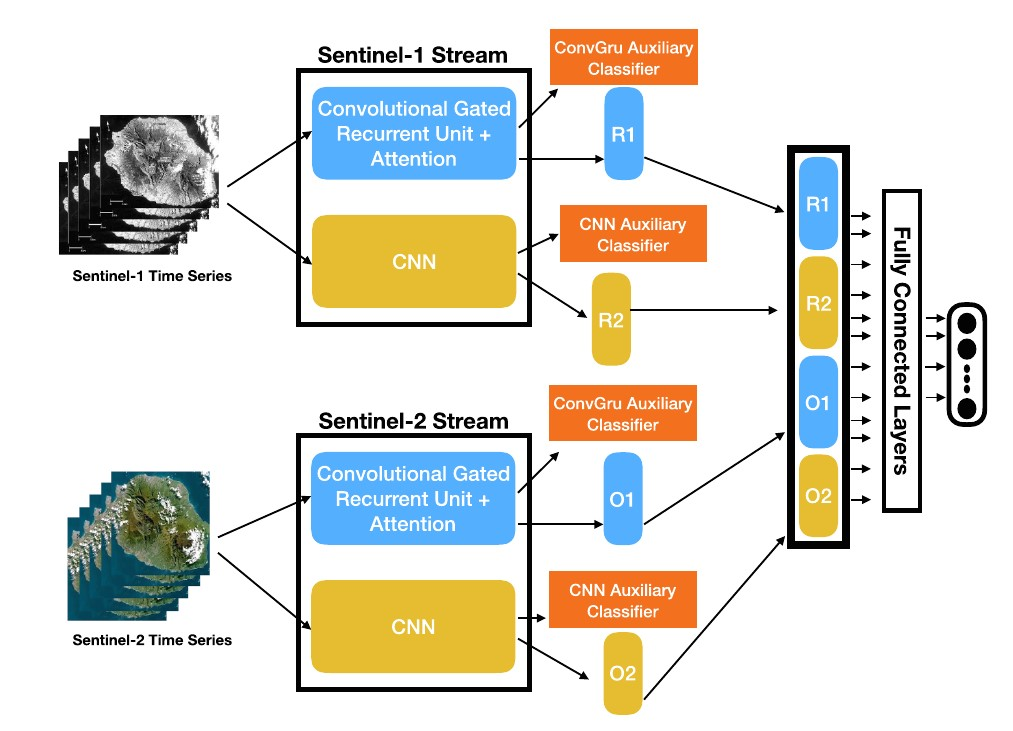
\includegraphics[width=0.8\textwidth]{pic/chap0101.jpg}
    \caption{模型结构}
    \label{fig:0101}
\end{figure}

每种数据源使用结构相同的stream. 每个stream有两个分支, 一个是convGRU分支和一个CNN分支. 在CNN分支中, 介绍了ReLU激活函数, 选择BN(batch normalization)的原因, Dropout的选择; 在convGRU分支中, 用GRU单元与LSTM对比, 说明GRU参数少, 计算量小的优点. 用内置了两层卷积的GRU单元, 并引入注意力机制作为convGRU单元. 模型训练部分主要介绍了提出的五个分类器以及损失函数的设计. 具体原理, 没有看明白.

\subsection{Experiments}
\subsubsection{Competin Methods}
将提出的算法与以下四个方法做对比:
\begin{itemize}
    \item 直接输入哨兵一号时序影像和哨兵二号时序影像的随机森林决策树算法, 记作$RF(S_{1},S_{2})$.
    \item 分别对哨兵一号时序影像和哨兵二号时序影像使用随机森林, 将两者分类结果做决策级的数据融合. 记作$RF_{LF}(S_{1},S_{2})$.
    \item 使用其他学者提出的convLSTM模型对每个数据源进行特征输出, 将两个1024维的特征串联得到2048维特征, 增加全连接层, 输出分类结果. 记作$2ConvLSTM$.
    \item 将TWINNS训练出特征使用随机森林分类. 记作$RF(TWINNS)$
\end{itemize}


\subsubsection{Experiments Setting}
主要包括CNN模型参数设置; 训练集, 验证集, 测试集制作; 实验平台CPU, 内存, GPU配置; 训练花费时间等.

\subsubsection{Ablation analysis}
理解Ablation(消融) analysis为对比实验. 主要通过实验说明模型结构的优越性.
\begin{quotation}
    \itshape
    比如说你为了提升baseline的性能, 给它加了两个模块A,B, 加完之后效果果然提高了很多. 于是你急急忙忙开始写论文, 写到你的贡献, 你给了两条:1.模块A, 2.模块B. 
    
    但是这样写有个问题:尽管AB同时加上去对模型有提升效果, 但是你并没有证明A、B两个模块分别都是有意义的. 所以为了验证A、B两个模块是不是真的都有用, 你需要做ablation study. 方法也很简单:
    \begin{itemize}
        \item 在baseline的基础上加上模块A, 看效果. 
        \item 在baseline的基础上加上模块B, 看效果. 
        \item 在baseline的基础上同时加上模块AB, 看效果. 
    \end{itemize}
    
    然后结果可能是, 实验1和实验2的结果都不如实验3, 那么说明AB都是有用的;然而也有可能你会发现实验1的结果和实验3一样, 甚至更好. 这就说明你的想法是有问题的, 模块B其实并没有起到作用, 提升只来自于模块A. 
    
    综上所述, ablation study就是你在同时提出多个思路提升某个模型的时候, 为了验证这几个思路分别都是有效的, 做的控制变量实验的工作. 
\end{quotation}

本文主要以三个点设计了对比试验:
\begin{itemize}
    \item 单独对哨兵一号时序影像和哨兵二号时序影像使用TWINNS模型. 验证模型对多源时序影像与单一时序影响的土地分类的精度. 分别命名为$TWINNS(S1)$, $TWINNS(S2)$.
    \item 对多源时序影像分别使用CNN和RNN, 记作$FullCNN$, $FullRNN$. 验证TWINNS模型是否优于两者.
    \item 验证所提出四个分类器对模型的作用, 将剔除分类器后的模型记作$TWI-NNS_{NoAux}$
\end{itemize}

\begin{table}[!htbp]
    \centering
    \begin{tabular}{c|p{2cm}|p{2cm}}
        \hline
                 & True & False     \\ \hline
        Positive & TP   & FP     \\ \hline
        Nagetive & FN   & TN     \\ \hline
    \end{tabular}
    \caption{二元分类}
\end{table}

分别可得到精度, 召回率, 准确率:
\[precision=\frac{tp}{tp+fp}\]
\[recall=\frac{tp}{tp+fn}\]
\[accuracy=\frac{tp+tn}{tp+fp+fn+tn}\]

多元分类评价指标中, 精度与召回率与二元类似, 其中第$i$类地物的精度与召回率指标为:
\begin{equation*}
    precision=\frac{a_{ii}}{\sum\limits_{k=1}^{r}a_{ik}}
\end{equation*}

\begin{equation*}
    recall=\frac{a_{ii}}{\sum\limits_{k=1}^{r}a_{ki}}
\end{equation*}



模型整体准确率计算公式为, 其中$N$为参与分类的像元总数:
\[accuracy=\frac{\sum\limits_{i=1}^{r}a_{ii}}{N}\]

改论文使用的其他两个分类精度评价指标:
\[F_{\beta}=(1+\beta_{2})\frac{precision\times recall}{\beta^{2}precision+recall}\]
\[F_{1}=\frac{2\times precision\times recall}{precision+recall}\]
\[p_{0}=accuracy\]
\[ p_{e}=\frac{\sum\limits_{i=1}^{r}[(\sum\limits_{m=1}^{r}a_{im})(\sum\limits_{n=1}^{r}a_{ni})]}{N^{2}} \]

\[ kappa=\frac{p_{0}-p_{e}}{1-p{e}} \]
\[
    kappa=\frac
    {N\sum\limits_{i=1}^{r}a_{ii}-\sum\limits_{i=1}^{r}[(\sum\limits_{m=1}^{r}a_{im})(\sum\limits_{n=1}^{r}a_{ni})]}
    {N^{2}-\sum\limits_{i=1}^{r}[(\sum\limits_{m=1}^{r}a_{im})(\sum\limits_{n=1}^{r}a_{ni})]}    
\]

$F\text{-}Measure$是$Precision$和$Recall$加权调和平均$kappa$用于一致性检验. $kappa$的公式推导与$F\text{-}Measure$的公式推导未知. 

此处作者得出两点结论:
\begin{itemize}
    \item 使用多源时序影像比单独时序影像效果好
    \item TWINNS(convRNN)比效果优于单一的CNN或是RNN
\end{itemize}

\subsubsection{Comparative evaluation}
不同方法和提出的TWINNS, 整体分类精度评价和每一类地物的混淆矩阵. 展示各种地物的分类结果图.

\subsection{个人总结}
Introduction部分, 从地球观测计划的高时空分辨率卫星影像为时序分析奠定了数据基础, 到单独哨兵一二号时序数据的研究应用, 再到多源影像优于单一源影像, 并且现阶段使用传统机器学习方法多源影像并未考虑数据之间关联性, 直接否决掉了机器学习算法, 引入深度学习. 

深度学习遥感影像分类多用RNN和CNN. 现阶段用结合两者优点的convRNN. convRNN用在单一时序影像. 多源时序影像只有CNN, 深度学习在多源影像潜力很大, 提出TWINNS为convRNN, 用在多源时序影像. 一要在不同源影像中互补, 二是可挖掘同源影像的时空数据关联. 

因此这两点一定要体现在模型与实验中.

本文研究地区有两个, 因此实验很多. 介绍模型方面, 主要为各个分支和损失函数和具体unit的优劣. 考虑到其未开源, 示意图不够细致, 只是展现了大体的思想. 但其引证其他文献对最后四个特征向量也是简单的串联, 这和在introduction中的批评他人对特征简单串联没有挖掘不同源数据间的关联形成矛盾, 当然也有可能是我并未细看其参考文献. 第二点时空数据关联可在convGRU单元中体现.

重点在于实验部分. 也是学习这种提出某类模型的论文写法. 重点有两个, 一是消融分析, 通过对模型某些结构的剔除来对比该模块对模型的作用, 相当于原理解释; 二是整体模型与其他方法或是其他深度学习模型的比较, 验证结果的优越性. 最终使用一系列分类精度评价指标, 如$kappa$, $accurracy$, $F\text{-}Measure$来评价模型. 也有混淆矩阵, 分类结果图等展示每个地物在不同方法下的分类结果. 

当然这些实验对比都是为了说明在introduction提出的不同源影像互补和挖掘同源影像的时空数据可更好用于分类. 
